\chapter{Implementation}
\label{ch:implementation}
From a practical point of view, the aim of this project was to create a working web application that also makes use of the best available development practices, well-designed architecture and is easy to maintain and extend in the future. The application is a relatively small-scale one, but it was developed with a future large-scale application in mind, that would allow many users to experience the application at the same time.

This chapter examines the implementation of the web application.

\section{Choice of Technologies}
\label{sec:choiceoftechnologies}
The application will be built using a set of front end and back end technologies. In this section will be justified the choice made in favour of each separate technology used in the project. 

\subsection{Front End}
The markup of the future application will be coded using HTML 5 \cite{documentation:HTML}. The application markup will be built using BEM front end development approach \cite{documentation:BEM}. BEM (short for "Block Element Modifier") is a popular semantic model for markup and a way to organise sections of a website into purposeful blocks and to optimise CSS. The idea behind is to logically break the HTML down into \emph{independent} blocks, which will allow arbitrary placement of the block anywhere on the page, including nesting the block inside another block. The approach can be  very beneficial for large websites, allowing the code to be reused across pages or even projects. However, a small project like the SureThing can also benefit from BEM by making use of independent, context-free CSS that can be easily amended in the future \cite{article:BEMForSmallProjects}.

CSS3 is used to define the visual presentation of the application. In general, CSS has certain limitations of its syntax capabilities. For example, it does not allow the use of variables, macros, mixins (reusable blocks of styles) functions and other features associated with object-oriented development, which inevitably leads to the creation of immensely repetitive stylesheets. In order to overcome those limitations, SASS preprocessor \cite{documentation:SASS} will be used in this project. SASS (short for Syntactically Awesome Stylesheets) is a powerful language that extends CSS with a choice of useful functionality, all in CSS-compatible syntax. Use of SASS would allow to make CSS code more efficient and easily maintainable. 

On the top of that, a popular CSS framework Bootstrap 3 \cite{documentation:Bootstrap3} will be used. Bootstrap provides a number of ready solutions for designing the layout of the future application. Therefore, the overall architecture of the markup will be defined by identifying BEM blocks and elements. This would bring structure into the code across all front end technologies used in the development. BEM blocks and elements will be complemented with appropriate Bootstrap classes in order to speed up the development process and make the application fully responsive.
 
JavaScript, specifically JQuery library \cite{documentation:jQuery}, will be used to add animations and improve overall user experience from using the application.  

In order to handle time-consuming and repetitive tasks on the front end side, the task-based command-line tool Grunt will be used. This software comes with a variety of plugins serving different purposes. For this project will be used \emph{grunt-sass} to compile SASS stylesheets into CSS complemented with \emph{grunt-watch} to allow continuous development, \emph{grunt-css} plugin to combine the all external CSS files into one and \emph{grunt-uglify} plugin in order to reduce the size of JavaScript files and speed up loading of the web page in a browser. This is a screenshot of running grunt for this project in terminal.

\begin{figure}[H]
	\begin{center}
		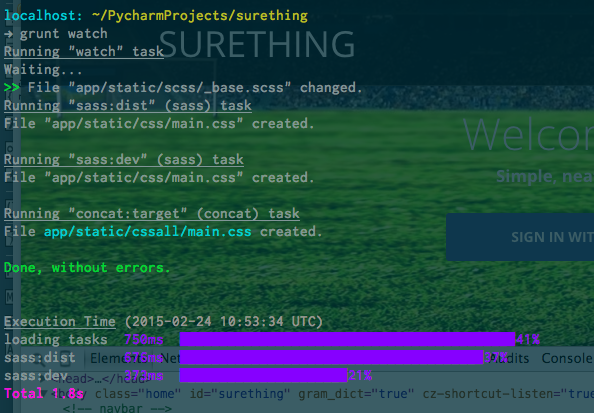
\includegraphics[width=.60\linewidth,natwidth=610,natheight=540]{impl/images/gruntInAction}
		\caption{Grunt running in terminal.} \label{fig:using:gruntInAction}
	\end{center}
\end{figure}
	
In addition, RequireJS  \cite{documentation:RequireJS}, a powerful asynchronous script loader will be used for effective management of JavaScript dependencies. It can load modules in asynchronous manner if desired and thus improve overall website performance.

\subsection{Back End}
For making reasonably accurate football results predictions the application requires latest footaball data. Live data would have to be frequently loaded into the system and processed in an appropriate way. Therefore, there would be a need for at least one separate module dealing with a third party football data API and containing business logic to manipulate the received data. The API wrapper is expected to be integrated into the web application, but separated from the presentation, it also has to be relatively easy to execute as a standalone module, encouraging a nicely decoupled design. Based on the above assumptions, Python was chosen as a primary back end language for this project being known as a language well suited to data manipulation.

The back end of the web application will be built using Python web framework Flask \cite{documentation:Flask}. It is a lightweight framework (the official name is "Python microframework") with a great choice of third-party libraries (e.g. Flask-SQLAlchemy or Flask-Login) that can extend the feature set of the framework core in various ways. Flask application is minimalist to begin with, but it can grow with the project needs. For the purpose of this project this is an advantage compared to the full-featured frameworks like Django that have a lot of functionality already built-in in the basic installation. In addition, availability of developer-friendly documentation and low learning curve makes Flask a short way to get a simple, Python-powered web site up and running. Therefore, Flask appears to be a great choice for a small project like SureThing. 

SQLAlchemy was chosen as database solution for this project \cite{documentation:SqlAlchemy}. This is a powerful database framework that supports several databases back ends and offers the high-level Object Relational Mapper (for short, ORM). Using ORM provides a great level of abstraction when working with databases. For example, SQLAlchemy uses classes that map to each table in a database. This means that the records interaction can be kept the same regardless of the underlying database system. This offers a lot of flexibility and, for example, allows to use different database systems for development and production environment. According to \cite{book:Grindberg2014FlaskWebDevelopment}, "Flask-Migrate extension, based on a migration framework Alembic and written by a lead developer of SQLAlchemy, provides a powerful solution to handle database alterations and make database schema updates easily manageable" 

\section{Application Architecture}
\label{sec:applicationarchitecture}
Application architecture is a base of a good quality software. The architecture of SureThing was from a big part dictated by the used framework, Flask, that uses a variation of MVC for Python called "MTV" (Model-Template-Controller). \cite{article:goodArchitecture} in his blog post describes this pattern in the following way:

\begin{quote}
"The template contains HTML content and presentation logic. It is written in a templating language ... It gets data from the view and outputs a web page. The view (also sometimes called “controller”), written in Python, is just glue code. It uses the web framework to put everything together. The model layer is essentially a persistence layer: its most important dependency is SQLAlchemy. The model knows how to save the data, constituting the most reusable code in the entire project."
\end{quote}

However, on the top of the standard MVC architecture SureThing requires few extra components to manage the loading of the data from an external source. Thus, this is the final structure of the architecture:

\begin{itemize}
    \item \textbf{Model Layer.} Contains Python classes that represent database models and related logic. According to \cite{article:goodArchitecture}, model layer "represents the essence of your system without the details of a user interface."
    \item \textbf{View Layer.} Holds association between URLs requested in the browser and Python functions or \emph{routes}. Routes are declared using an appropriate function decorator, for example:

\begin{figure}[H]
    \begin{center}
        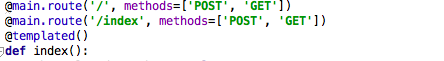
\includegraphics[width=.40\linewidth,natwidth=610,natheight=642]{impl/images/indexPageRoute}
        \caption{Index page route example.} \label{fig:using:indexPageRoute}
    \end{center}
\end{figure}     
        
    \item \textbf{Template Layer.} This is the mediator layer between an HTTP request and the application logic. It consists of a number of Jinja2 templates holding only     presentation logic. 
    \item \textbf{External Services Layer} \cite{article:goodArchitecture}. Contains API wrapper class that accesses and manipulates live football data. In general, the functionality of the application can be further extended in many ways. In the future, Football-API might not be the only external source of information. The project might make use of another third-party API or even web scrapping. Eventually, all additional modules related to the interaction with external sources of data will become part of this layer.
    \item \textbf{Threading.} The application requests live football data frequently. Loading the data is a costly I/O operation that may become a bottleneck. This component defines a class \emph{DataUpdateThread} that takes care of writing the data to the server every 100 seconds. This task is carried out in a separate thread. 
\end{itemize}

During the development process, a lot of effort was put into keeping the Template Layer thin as possible in order to reduce the loading time in the browser and improve the overall performance of the application.

\section{Implementation Processes}
In this section a number of  various techniques and tools used during application development will be described and explained. 

\subsection{Application Factory}
The use of factory pattern is crucial to a Flask application. For example, SureThing app defines various configurations to be used in different environments (development, testing, production). However, because the application instance is created in the global scope, there is no way to apply those configurations. As described in the \cite{book:Grindberg2014FlaskWebDevelopment}, the problem is that "by the time the script is running, the application instance has already been created, so it is already too late to make configuration changes." To get around this problem a creation of the application was moved into a separate function, \emph{create\_app()}. The name of configuration name is passed into the function as a parameter. This solution also allows us to create multiple instances of the application and makes testing of various confurations easier.\cite{documentation:FlaskApplicationFactories} 

\begin{figure}[H]
	\begin{center}
		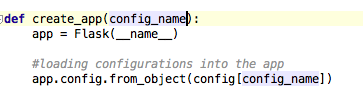
\includegraphics[width=.40\linewidth,natwidth=610,natheight=642]{impl/images/createApp}
		\caption{Function responsible for creation of the application.} \label{fig:using:createApp}
	\end{center}
\end{figure}

\subsection{Blueprints}
Blueprints are related to the View Layer introduced in the section Application Architecture \cite{sec:applicationarchitecture}. A large application is divided into smaller parts and each part is implemented with help of a blueprint. This concept helps to develop a \emph{modular} web application. SureThing was divided into two parts: \emph{main} and \emph{auth}. \emph{auth} holds the endpoints associated with the authentication and user profile related tasks, for example \emph{login()}, \emph{edit\_profile()}. On the other hand \emph{main} is in charge of the rest of the application. Please notice how those different blueprints are registered on the application instance inside the \emph{create\_app()} function:

\begin{figure}[H]
	\begin{center}
		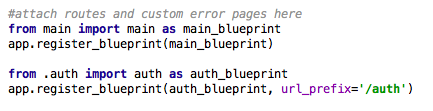
\includegraphics[width=.60\linewidth,natwidth=610,natheight=642]{impl/images/blueprintsRegistration}
		\caption{Blueprints registration.} \label{fig:using:blueprintsRegistration}
	\end{center}
\end{figure}

\subsection{Database Migrations}
The database scheme for this project was designed in an iterative way, models and relationships between them were added gradually as the application was growing. Therefore, it was crucial to find a tool that allows effortless updates of the database. To manage frequent database updates was used Alembic database migration tool that was developed specifically by Mike Bayer, the author of SQLAlchemy. The tool can be added to Flask as an external plugin, Flask-migrate. After installation and initial configuration of the plugin, it allows to migrate the database with two simple commands to be subsequentially run in the terminal: \emph{db upgrade} and \emph{db migrate}. Alembic makes migration easier and prevents the developer from the necessity to delete and recreate the database each time there is a need for migration.

\subsection{Version Control}
Git version control system was used throughout the development process. Git is known for being a very useful tool for collaboration across teams of developers. However, it has also many benefits for a solo developer. For example, it helps to track changes and restore previous versions of a project, as well as view the code at any point in the past. The project codebase was uploaded to GitHub that is \cite{wiki:GitHub} "a web-based Git repository hosting service, which offers all of the distributed revision control and source code management (SCM) functionality of Git as well as adding its own features... (It also) provides web-based graphical interface". For this project GitHub issue tracker was used as a "to-do list" to keep the record of tasks ("issues" in GitHub terminology) that needed to be completed in each agile iteration. Custom labels were used to distinguish different types of issues in the GitHub issue tracker, for example, performance, design, bug, optional tasks, etc. 

\begin{figure}[H]
	\begin{center}
		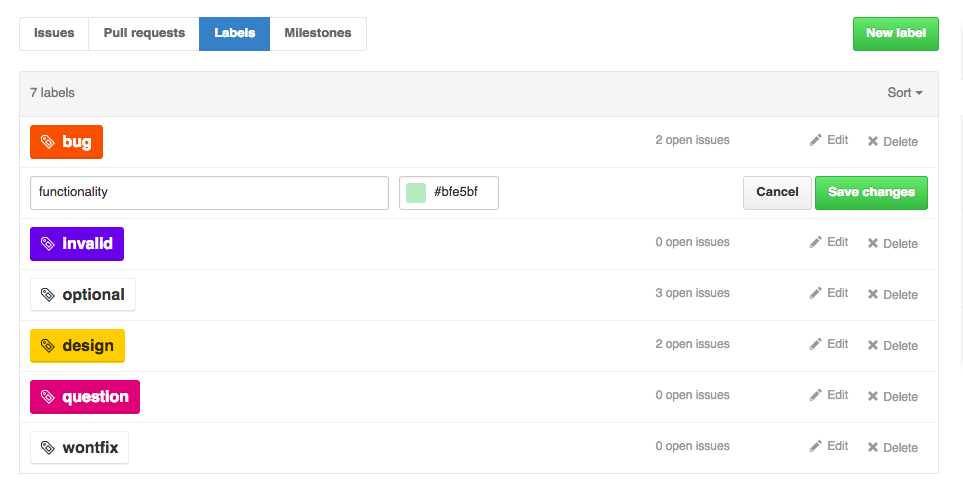
\includegraphics[width=.90\linewidth,natwidth=610,natheight=642]{impl/images/githubLabelsChoice}
		\caption{GitHub. Custom labels.} \label{fig:using:githubLabelsChoice}
	\end{center}
\end{figure}

GitHub also allows the users to filter out the issues of a similar type, based on the assigned label.

\begin{figure}[H]
	\begin{center}
		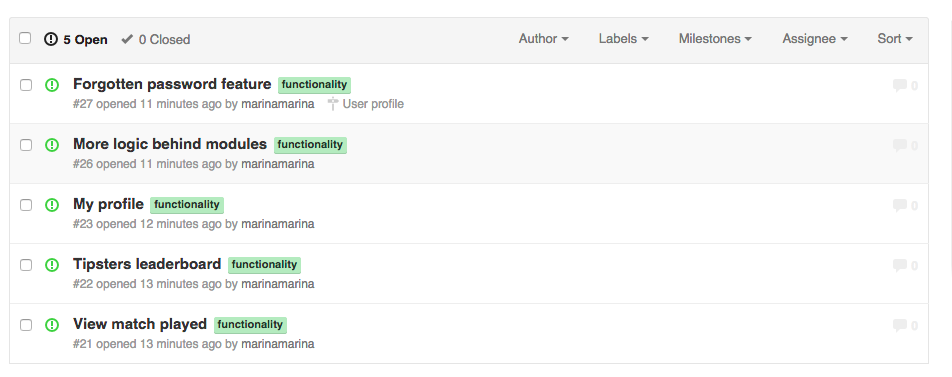
\includegraphics[width=.90\linewidth,natwidth=610,natheight=642]{impl/images/githubFunctionalityIssues}
		\caption{GitHub. Issues related to the functionality of the application.} \label{fig:using:githubFunctionalityIssues}
	\end{center}
\end{figure}

Critically speaking, I missed the option to assign issues various level of importance and order the issues based on their priority.

\subsection{Own Validation in Forms}
Flask-WTF is a Flask extension that offers integration with WTForms and it was used to handle forms in this project. In order to make sure the application is secure, the validation has to be implemented preferably on the server side or both on the client- and server-side of the application. WTForms has many built-in validators that can simplify developer's life. For example \textbf{DataRequired} makes the input field mandatory, \textbf{Email} checks that the provided input is a valid email address, \textbf{EqualTo} helps to ensure that the passwords in the fields "Password" and "Confirm Password" supplied during the user registration are identical. However, sometimes the built-in functionality does not cover all the application needs. In that case, there is an option to create a custom validator that is a basically a Python function returning another function (a validator) that throws an exception every time the user violates the prescribed validation rule. Custom validators can be imported into the module describing forms and used in the same way as a built-in validator would be used. I have separated the validators out into a separate module. The set of custom validators can be further extended, however, there is just one at the moment: \emph{validator\_user\_already\_registered()}. 

\begin{figure}[H]
	\begin{center}
		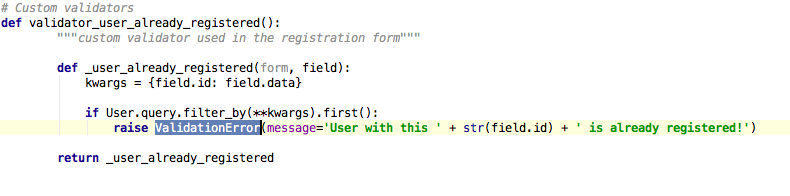
\includegraphics[width=.90\linewidth,natwidth=610,natheight=642]{impl/images/customValidator}
		\caption{Validator function that checks if user with this username has already been registered with the SureThing application} \label{fig:using:customValidator}
	\end{center}
\end{figure}

In the example above the validator function checks if a user with provided username is already in the database. If the user is found, the ValidationError exception is thrown and the new user is prevented from submitting the form.

\subsection{Custom Macros}
Jinja2 is a default template engine that comes in one package with Flask. It is also one of the most widely used template engines for Python. In order to add some extra presentation logic to our application, custom macros can be used. Jinja2 macro is simply a template function that can be used within HTML in order to avoid developers writing repetitive code. For this project I found macros extremely useful. Custom macros were separated out into a separate template file \_macros.html.

One of the example usages was rendering form fields. Each form field related macro contained a piece of HTML code specifically designed for forms in this application, as well as logic for dispaying error messages. Among this type of macros can be named \emph{render\_field(field)}, \emph{render\_checkbox(field)}, \emph{render\_submit\_field(field)}. Some of those macros needed to be adjusted to enable their usage in a specific view. These are the examples of such "adjusted" macros: \emph{render\_submit\_field\_match\_preview(field)}, \emph{render\_embedded\_field(field)}. For example, \emph{render\_field} takes care of rendering any standard input field accross the application, whereas \emph{render\_embedded\_field(field)} manages rendering an input field embedded within a prediction module on the Upcoming Match View. 

Another macro, \emph{teamkitimage(match, home=1)} renders an image representing a football club. Based on the provided arguments, the function displays an image of a home or away team kit for a specific club. 

\subsection{Exceptions}
The application will make use of Exceptions in order to identify and manage failures when making an API call over HTTP. The FootballAPIWrapper class has a private method that calls the API and collects the data in a JSON format from the remote server: \emph{\_call\_api(action=None, **kwargs)}. The method takes into account the possibility of errors occuring during code execution. When the program calls the API, either JSON data is returned or an Exception is thrown. 

As it can be seen from the method definition above, one of the required parameters is \emph{action} that is set to None, unless the value is passed in during the method call. Action is a string that needs to be added to the base url in order to indicate the set of data that is being accessed. Specifying the action is required by the API and the possible values of the parameters (actions) are: competition, standings, today, fixtures, commentaries. For example action \emph{today} will returns the matches scheduled today. The \emph{\_call\_api} method will raise an Exception, if the action is not being supplied. Various exceptions are thrown when the program is attempting to connect to the remote server \cite{article:httpRequestsExceptions}. Python library \emph{requests} is used to take care of this type of errors. \cite{documentation:PythonRequests} If the domain name does not resolve, the HTTP request will fail before we establish connection. In that case, the program will throw a \emph{requests.exceptions.ConnectionError}. If the remote server is not functioning or the request is structured incorrectly, the server will respond with an bad response status code and the \emph{\_call\_api} method will raise a \emph{requests.exceptions.HTTPError}.

\subsection{Integration with third-party API}
Many production Python web applications rely on external application programming interfaces (APIs). API can be also reffered to as "third party services" or "external platform".\cite{apiintegration}  SureThing requires constant access to current football data. After choosing an appropriate API, it has to be integrated into the application. 

There is a variety of tools available for developers for accessing web APIs. Those three options were considered when choosing an appropriate tool:
	
\begin{itemize}
	\item Helper library (such as Runscope or Apiary)
	Using a helper library has an overhead of learning how to use another piece of software.
	\item urllib2, standard Python module
	\emph{urllib2} module offers very simple implementation and provides most of the required HTTP capabilities, but the API is thoroughly broken and features critical for performance are missing, for example connection re-using/pooling. 
	\item urllib3
	\item requests, another Python library for handling HTTP requests. It offers a lot of control over the HTTP calls through the use of its powerful features.
\end{itemize}
		
After some experiments with other urllib2, urllib3 and requests, \emph{requests} was chosen as the libarary for this project.
		
All interaction with the Football-API, including processing the received data, was separated out into a module \emph{football\_api\_wrapper\.py} or just "wrapper" for short. This module contains only one class, FootballAPIWrapper. Fields of the class accomodate the key elements of the interaction with the API that will be re-used in different methods of the wrapper, for example base url, path to the data directory.
	
\begin{figure}[H]
\begin{center}
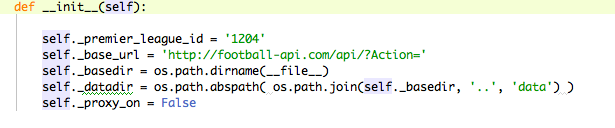
\includegraphics[width=.90\linewidth,natwidth=610,natheight=642]{impl/images/footballApiWrapperFields}
\caption{Football API wrapper, fields} \label{fig:using:footballapiwrapperfields}
\end{center}
\end{figure}
	
To get the response from Football-API takes about 11s, therefore it is nessessary to move the API calls into a task queue so they do not block the HTTP request-response cycle for the rest of the web application.

\subsection{Visual Effects}
Various visual effects were implemented with the help of jQuery, AJAX and the Flask-SocketsIO. 

A good example is an alert dismissal. SureThing generates many alerts that give the user feedback with regards to the action they have just taken. User has to dismiss the alert manually each time. To avoid this extra thing for a user to do, the alerts are removed from the page using jQuery fadeOut animation effect.

picture

New message


\subsection{Responsive Design}
The application is fully responsive. 
see Appendices


\section{Features Implementation}
In this section will be described the technical details of the project implementation. Each susbsection is bound to the high level feature of the application, as indroduced in the chapter "Requirements Analysis" \ref{sec:functionalrequirements}.

\subsection{Authentication and User Profile}

The application requires authentication functionality. In order to simplify the development process, one of the useful Flask's extentions, Flask-Login, was used to handle the common tasks of logging in and out, as well as new users registration. For the new users the application sends an email with verification token, expecting the user to confirm their email address. 

\subsection{Matches Overview}
Matches overview is a view diplayed on the main page of the application. It contains a list of upcoming and played matches.

\begin{figure}[H]
	\begin{center}
		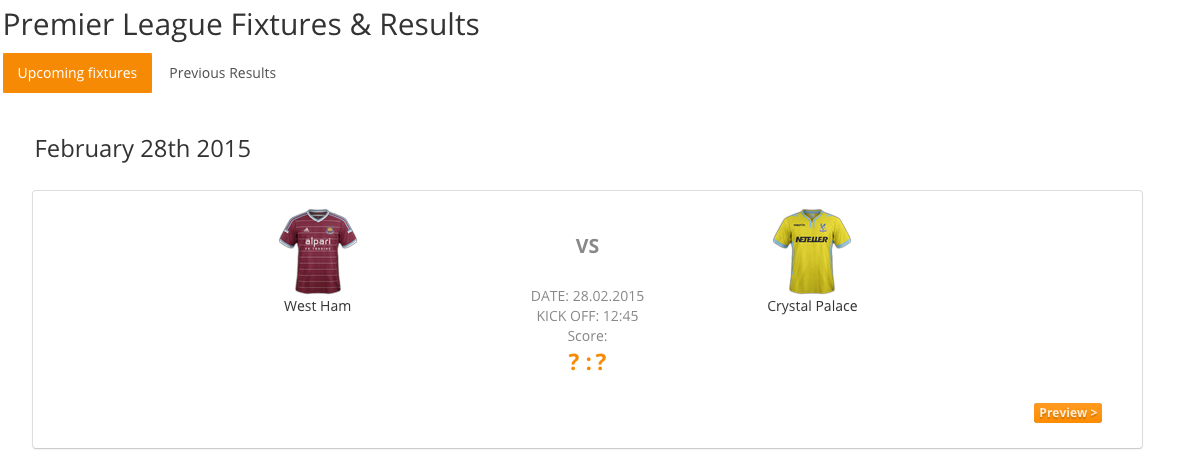
\includegraphics[width=.90\linewidth,natwidth=610,natheight=642]{impl/images/matchesOverviewExample}
		\caption{Matches Overview} \label{fig:using:matchesoverview}
	\end{center}
\end{figure}

\subsubsection{User Journey}
On the main page of the application user can see a list of upcoming matches. Above the list can be found simple navigation allowing to switch between lists of unplayed and played matches. The overview displays the most basic information about each match, such as names of teams participating in the match, kick-off date and time. On the right hand side of each list item there is a "Preview" button for an upcoming match and a "View Stats" button for a played match. By clicking those buttons user can navigate to views with more detailed information about the match. 

\subsection{Prediction}
The implementation of the prediction feature was already outlined in the chapter "Requirements Analysis", subsection "Definitions" \cite{subsec:definitions}. In this subsection I would like to decribe this key feature of the application in more detail. The application has three levels of prediction settings (weights). Firstly, it is the "default prediction settings" - a set of weights recommended to new users by the system. Once the user is registered with the application, they can set their own set of weights that will override the default settings. From the moment those weights are saved in the database, they will apply to every newly saved match. The application also allows users to set match specific settings that will only apply to one match. 
 


how the overall prediction is calculated, weighted prediction

\subsection{Upcoming Match View}
\label{subsec:implementupcomingmatchview}
Implementation of this view was one the most complex development tasks of the whole project.

\subsubsection{User journey}
\label{subsec:upcomingmatchviewuserjourney}
The user can navigate to this view either from the matches overview on the main page or from the dashboard (if the match has already been saved to the dashboard).

 If the user is coming to the upcoming match preview from the \emph{main page}, it will display the match header (containing general information about the teams, last played game, match kick-off time and date, etc.), a list of prediction modules and a \emph{prediction value} for each module calculated based on the relevant statistics for each of the teams. This information should be sufficient for the user to decide, whether it is worth saving the match to the dashboard for a latter revision. An unauthorised user would be able to see the same overview, but the "Save" button will be disabled. 

\begin{figure}[H]
	\begin{center}
		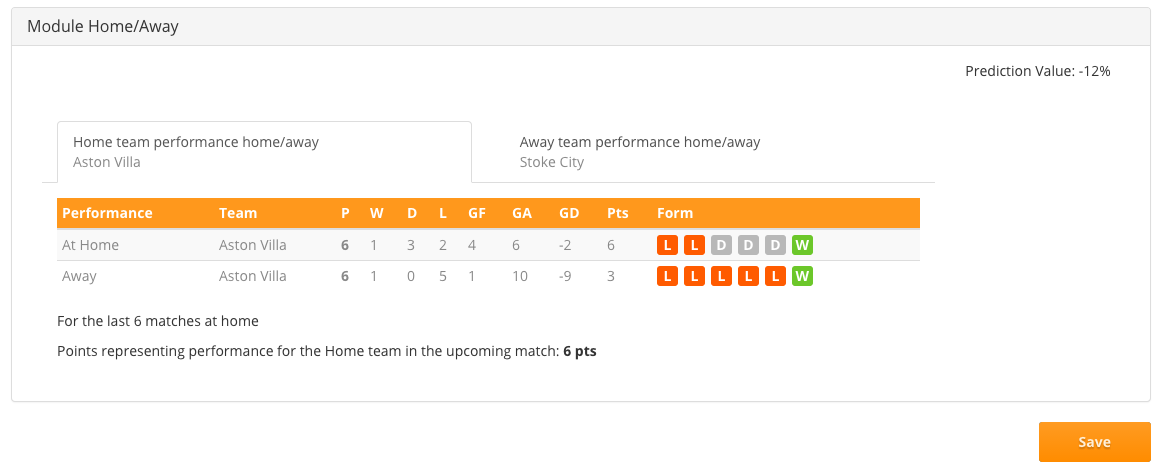
\includegraphics[width=.90\linewidth,natwidth=610,natheight=642]{impl/images/matchoverviewex_from_main_page}
		\caption{An example of a prediction module in the Match Preview, user navigated from the main page.} \label{fig:using: matchoverviewex_from_main_page}
	\end{center}
\end{figure}

If the user comes to the upcoming match preview from the \emph{dashboard}, they will be able to see more information related to the actual result prediction and betting.
First of all, in each prediction module they will see an input fields for setting match specific prediction weights. Secondly, they will see a user hunch module. Finally, at the very bottom of the overview they will see calculated prediction result and two buttons - one to save the match specific settings and another to commit the bet.

\begin{figure}[H]
	\begin{center}
		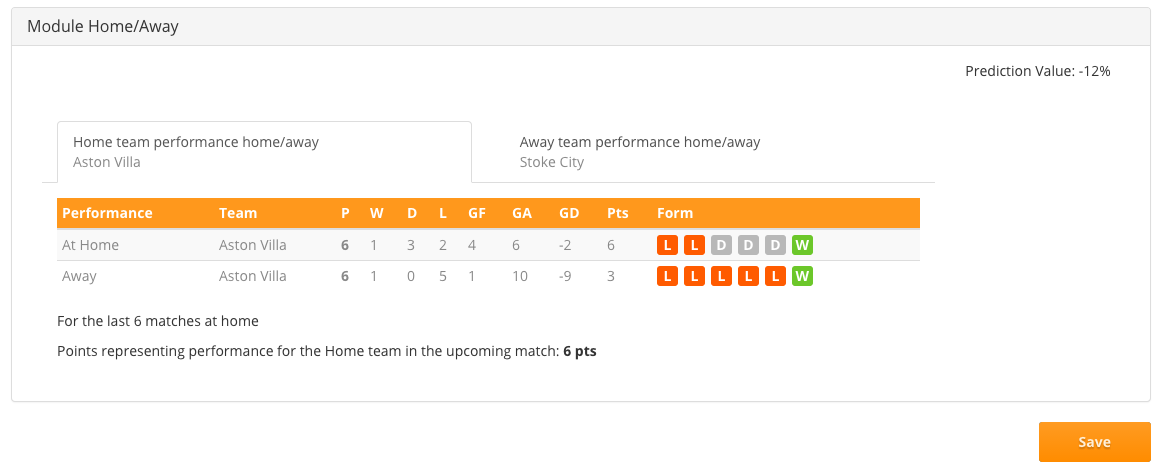
\includegraphics[width=.90\linewidth,natwidth=610,natheight=642]{impl/images/matchoverviewex_from_main_page}
		\caption{An example of a prediction module in the Match Preview, user navigated from the dashboard.} \label{fig:using: matchoverviewex_from_main_page}
	\end{center}
\end{figure}


 most Explain how was implemented user hunch: combination of Flask Ajax and Sockets IO!!!
 
\subsection{Played Match View}
\label{subsec:playedmatchview}

\subsection{Possible Future Enchancement}
\label{subsec:enchancement}

Although, one of the key features of the application is to try not to overhelm the user with statistics, as opposed to many football stats websites, this view would need a little bit more additional information to complete the big picture.

\section{Application Performance}
sockets, threads
multithreading
how I fixed performance on Match.update\_all\_matches

\subsection{Deploying the Application}
Cloud Deployment is the most recent trend in application hosting. The formal name of this technologu is Platform as a Service (PaaS).  In the PaaS model, a service provider offers a fully managed platform in which applications can run.

\section{Conclusions}
The main conclusions for this chapter.